\section{Fourier Transformation}
Our goal is to decrease the intensity of the spyders and speckles in the data. In our data from HD142527 the main disturbing effects are the spyders. With the transformation to the $r$-$\varphi$ plane the spyders now are parallel to the $r$-axis. When comparing different data sets from the same observation we find that the spyders change there position, but the distance between them stays the same. It is a periodic pattern. This brings up the idea, if the spyders are represented by a set of frequencies in the frequency plane. If this is the case, the suppression of some of the frequencies in the frequency plane would result in a suppression of the spyders in the image plane. The advantage of this method would be that it could be applied to the complete data set and one can ignore the fact that the spyders wander along the $\varphi$-axis. Also we should be able to suppress the spyders without destroying the information below them.\\
In the following we are going to investigate the properties of a Fourier transformation on some specific image structure as lines, beams and point-like sources.\\

\subsection{Lines and Beams}
\label{FFT_Lines_Beams}
We first want to investigate the effect of some simple signals in the image plane on the frequency plane. We choose these signals similar to the shape of the spyders or to the shape of a potential exoplanet, with the goal to identify similar characteristics in the frequency plane of the data.\\
Firstly, we transform a single line (has the width of one pixel) in vertical or horizontal direction to the Fourier plane. A single line in vertical direction ($y$-axis) means that we have a constant signal along the $y$-axis, but we have a non-constant signal in $x$ direction, namely a one pixel wide peak at the $x$ position of the line. So we expect that all $y$-axis frequencies in the Fourier transformed image to be zero, this means that only at $y$ frequency zero we have non-zero values which describe the periodicity in $x$ direction.\\
As we can see from figure \ref{fig:fft_line} the transformation of a single line results into a single line in the frequency plane. The line in the frequency plane is perpendicular to the line in the image plane and is located in the center. This confirms our expectations.\\
Since we plot our results with a logarithmic scale, we need to keep in mind that $\log(0) = -\infty$ . In order to be able to plot our results we added a small value $\epsilon$ to our Fourier transformed results just before plotting.
\begin{figure}[H]
	\centering
		\subfigure[]{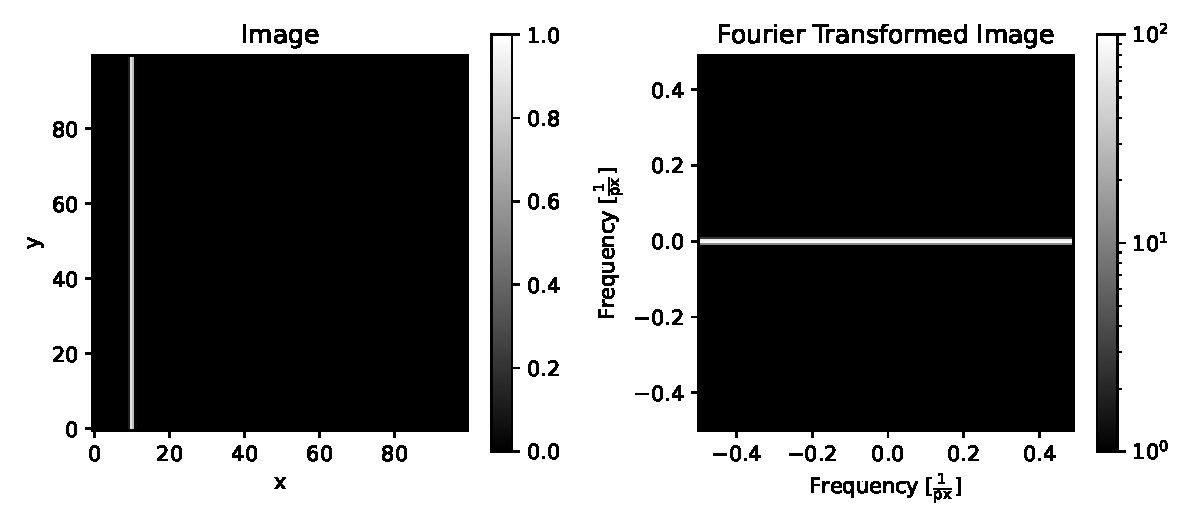
\includegraphics[width=1.0\textwidth]{pics/fft_simulationoneline.pdf}}
		\subfigure[]{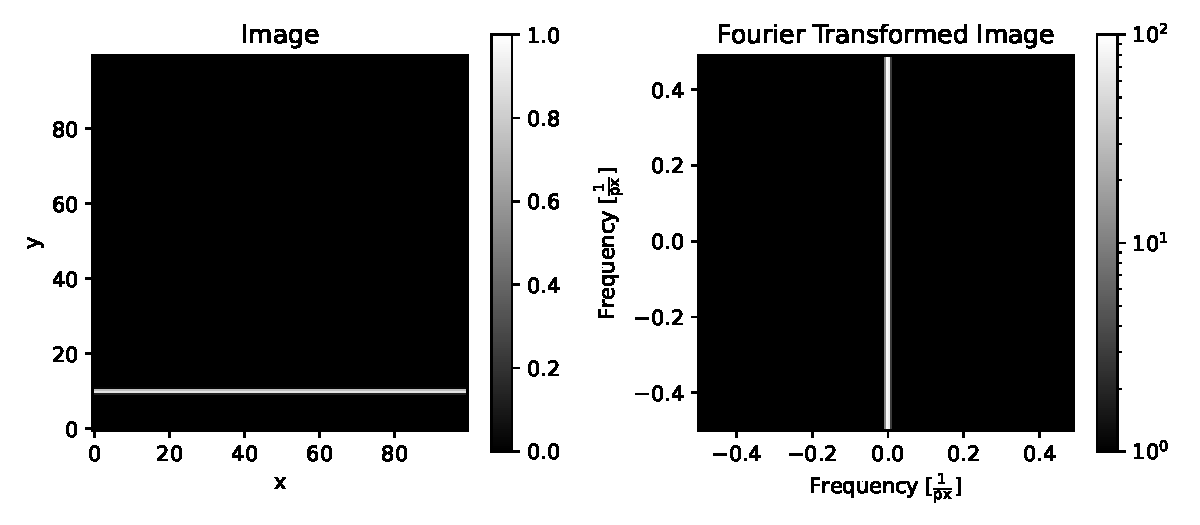
\includegraphics[width=1.0\textwidth]{pics/fft_simulationoneline_horizontal.pdf}}
\caption{The image of a vertical line (a) and of a horizontal line (b) (images on the left side) are transformed to the frequency plane (images on the right side).}
\label{fig:fft_line}
\end{figure}
To explore the frequency plane further we plot the intensity at $y$ frequency equals zero along the $x$ frequency axis (frequency plane of image shown in figure \ref{fig:fft_line} (a)). This describes the periodicity of the image in horizontal direction. As we see in figure \ref{fig:fft_line_cut} the intensity along this axis is constant.
\begin{figure}[H]
	\centering
		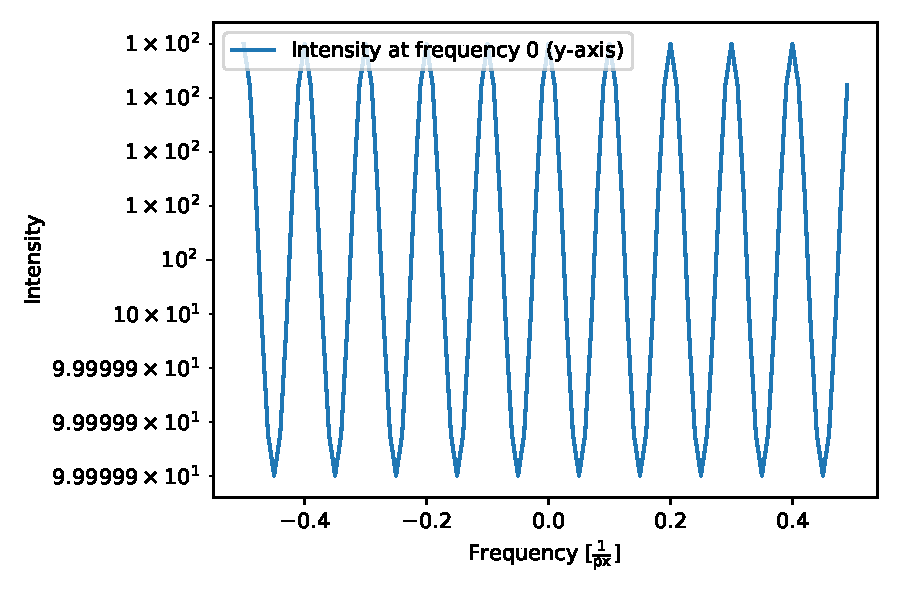
\includegraphics[width=0.8\textwidth]{pics/fft_simulation_cutoneline.pdf}
		\caption{The intensity of the Fourier transformed image in figure \ref{fig:fft_line} (a) at y frequency equals zero.}
		\label{fig:fft_line_cut}
\end{figure}
As a next step we want to find out what happens, if we insert a periodic signal into the image plane in the form of equally spaced lines. Figure \ref{fig:fft_lines} shows an image where there are several vertical lines with a spacing of 20 pixels. As in the case of the single line the image is constant in $y$ direction and so all vertical frequencies are assigned zero. In $x$ direction the lines create a periodic signal with frequency $\frac{1}{20} = 0.05 \frac{1}{\mathrm{px}}$. On the right side of figure \ref{fig:fft_lines} we see the fourier transformation of the image with the equally spaced lines and figure \ref{fig:fft_lines_cut} shows a horizontal cut through the center. We see that only the pixels at $0.05n \frac{1}{\mathrm{px}}$ $\forall n \in \{0, 1, 2, ...\}$ are non-zero.
\begin{figure}[H]
	\centering
		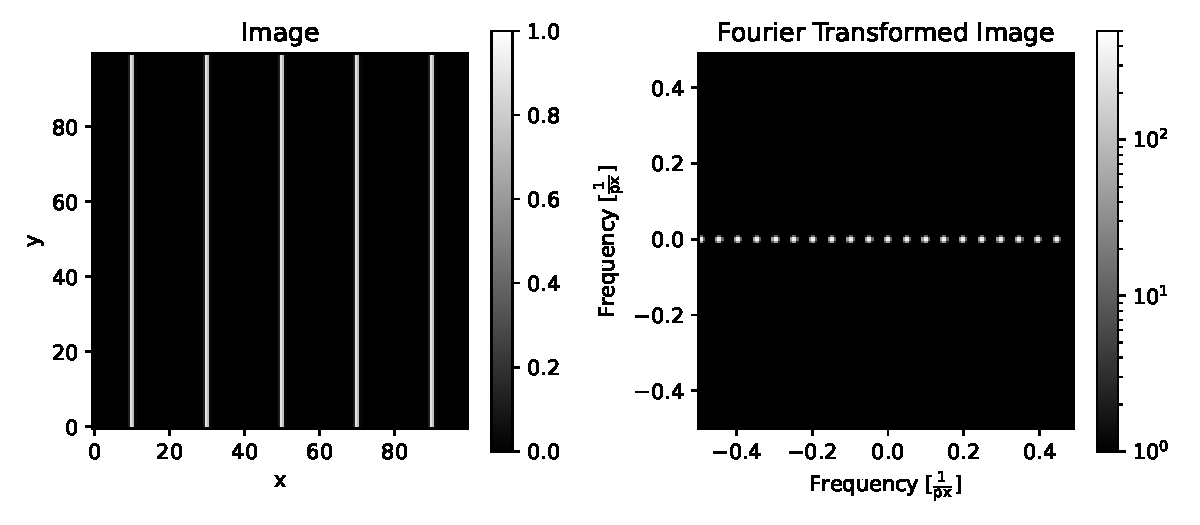
\includegraphics[width=1.0\textwidth]{pics/fft_simulationmorelines.pdf}
		\caption{The image with several equally spaced one pixel thick lines on the left is transformed to the frequency plane, see image on the right.}
		\label{fig:fft_lines}
\end{figure}
\begin{figure}[H]
	\centering
		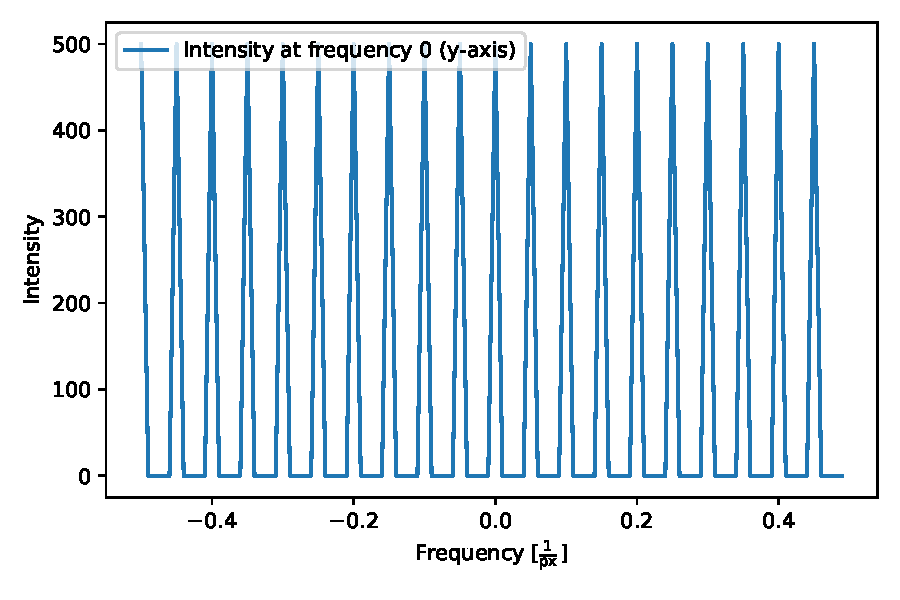
\includegraphics[width=0.8\textwidth]{pics/fft_simulation_cutmorelines.pdf}
		\caption{The intensity of the Fourier transformed image in figure \ref{fig:fft_lines} at y frequency zero.}
		\label{fig:fft_lines_cut}
\end{figure}
In the appendix \ref{almostPeriod} we show, what happens if one line in the periodic image is missing and thus the signal is not completely periodic. We find that the treshold raises up to a higher value.\\
The spyders are not lines, but they have also an expansion into the horizontal, so we are also interested to see the Fourier transform of a single beam. We investigate the image of a beam (stair function) with a width of 10 pixels, placed at $x=10$. Figure \ref{fig:fft_beam} shows the corresponding image and its Fourier transform. As with the lines the only frequencies in the frequency plane with a non-zero value are along the $y=0 \frac{1}{\mathrm{px}}$ frequency axis. Figure \ref{fig:fft_beam_cut} shows this axis in more detail. In contrast to the frequency plane of the line we have a signal which is stronger for central frequencies and decreases slightly for larger frequencies. Additionally we have strong minima at $0.1 n$ $\forall n \in \mathbb{N}$, where the position of the minima is given by one over the width of the beam.
\begin{figure}[H]
	\centering
		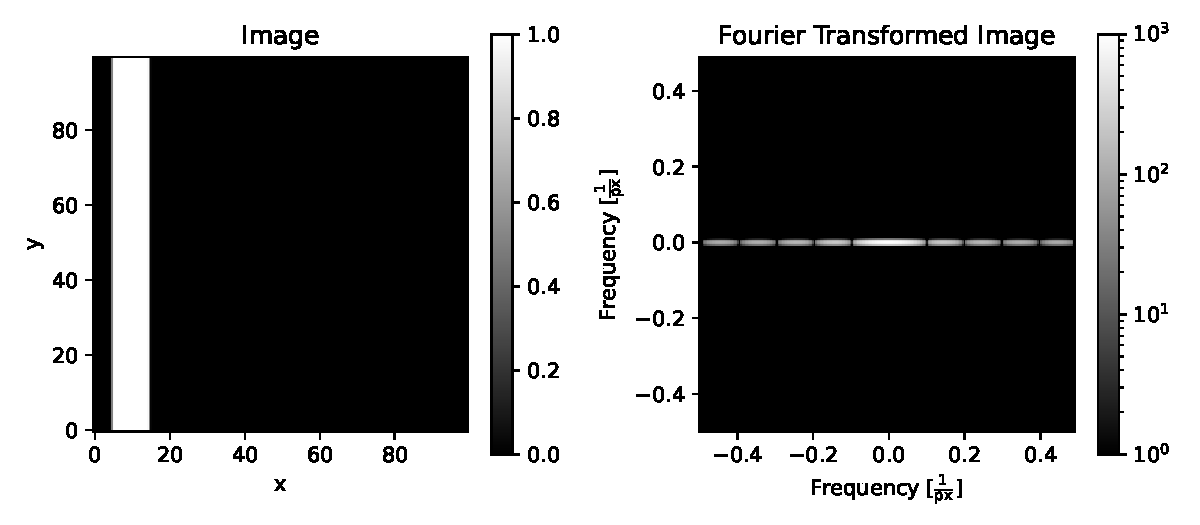
\includegraphics[width=1.0\textwidth]{pics/fft_simulationonebeam.pdf}
		\caption{The image of one 10 pixel thick beam on the left is transformed to the frequency plane, see image on the right.}
		\label{fig:fft_beam}
\end{figure}
\begin{figure}[H]
	\centering
		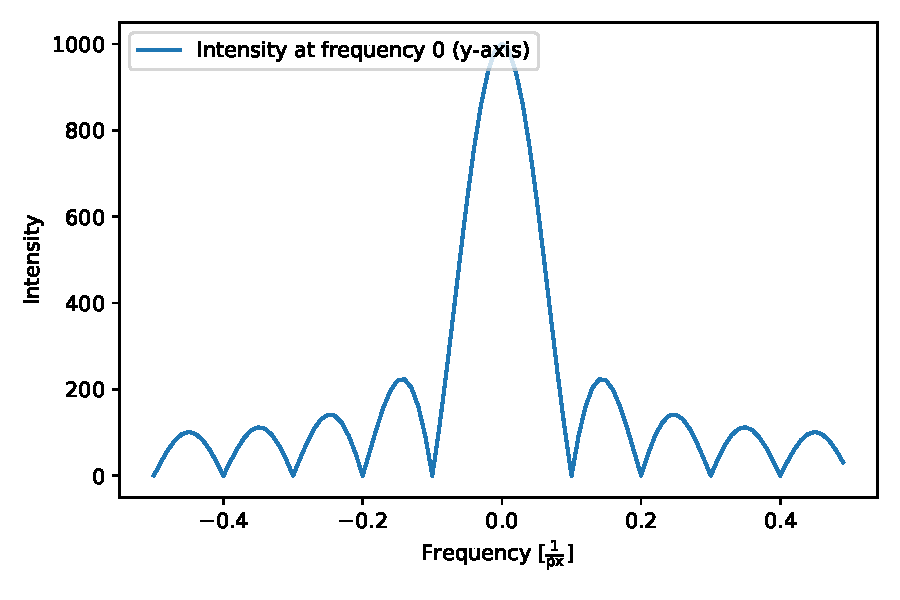
\includegraphics[width=0.8\textwidth]{pics/fft_simulation_cutonebeam.pdf}
		\caption{The intensity of the Fourier transformed image in figure \ref{fig:fft_beam} at y frequency zero.}
		\label{fig:fft_beam_cut}
\end{figure}
As before with the lines we have a look at what happens if we have several of this beams, again equally spaced with a spacing of 20 pixels. We find that this image, lets call it $h(x)$, is a convolution of the image with the equally spaced lines $f(x)$ and the image with the single beam $g(x)$, namely
\begin{equation}
	h(x) = (f * g)(x) = \int_{\mathbb{R}^n} f(\tau)g(x-\tau) \mathrm{d}\tau .
\end{equation}
From the convolution theorem we find that for the Fourier transform it yields:
\begin{equation}
	\mathfrak{F}\{h(x)\} = \mathfrak{F}\{(f * g)(x)\} = (G \cdot F)(\mu),
\end{equation}
where $G(\mu)$ and $F(\mu)$ are the Fourier transforms of $g(x)$ and $f(x)$ \cite{ImageProcessing}. This means that the Fourier transform of the image with the several beams is given by the multiplication of the Fourier transform of the image with the equally spaced lines and the image with the single beam, which can be seen in figure \ref{fig:fft_beams_cut}. Around the center frequency we have some peaks separated by $0.05 \frac{1}{\mathrm{px}} = \frac{1}{20} \frac{1}{\mathrm{px}}$ which describes the separation between the beams of $20$ pixels. This peaks are surrounded by other peaks which are separated by $0.1 \frac{1}{\mathrm{px}} = \frac{1}{10} \frac{1}{\mathrm{px}}$ which describes the width of the beams of $10$ pixels.
\begin{figure}[H]
	\centering
		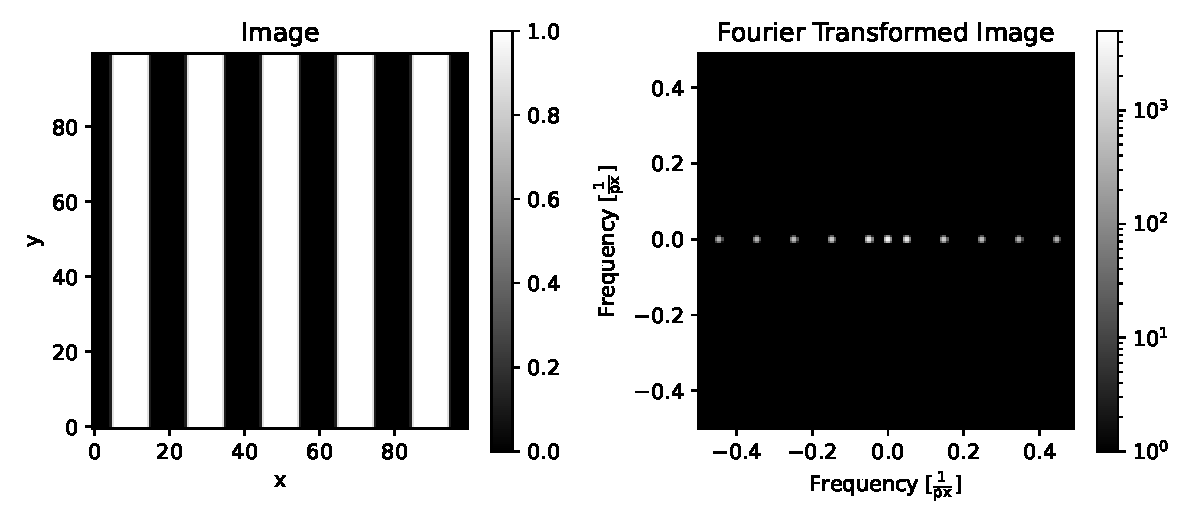
\includegraphics[width=1.0\textwidth]{pics/fft_simulationmorebeams.pdf}
		\caption{The image of several equally spaced 10 pixel thick beam on the left is transformed to the frequency plane, see image on the right.}
		\label{fig:fft_beams}
\end{figure}
\begin{figure}[H]
	\centering
		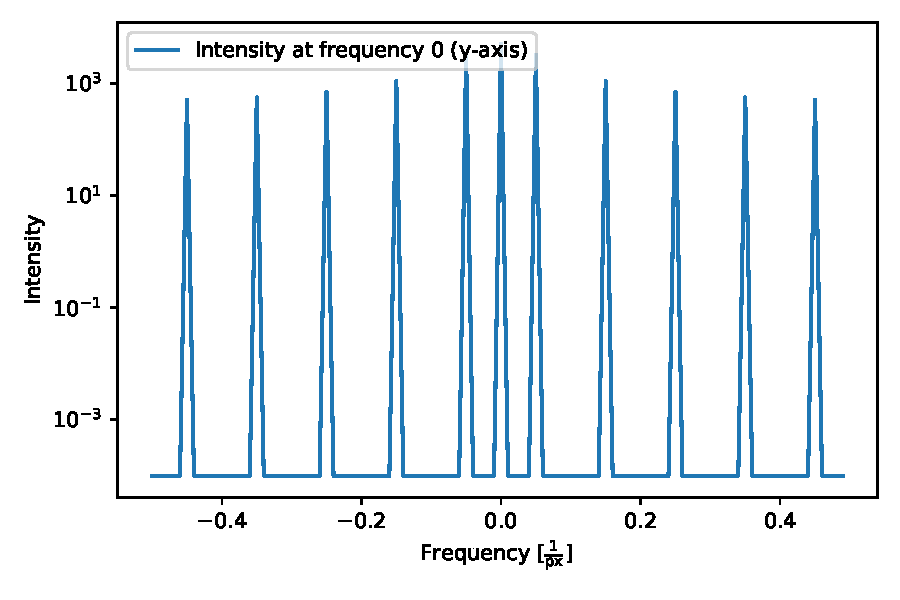
\includegraphics[width=0.8\textwidth]{pics/fft_simulation_cutmorebeams.pdf}
		\caption{The intensity of the Fourier transformed image in figure \ref{fig:fft_beam} at y frequency zero.}
		\label{fig:fft_beams_cut}
\end{figure}

\subsection{Gaussian Beams}


\subsection{Point-Like Sources}
In order to make sure that we are not going to suppress the signal of point-like sources as exoplanets we need to know how their signal is going to look like in the Fourier space.\\
We investigate the signal of a Gaussian point source and of a point spread function (PSF). A PSF describes how a point source looks like after it has gone through an imaging system \cite{PSFwiki}, which is in our case the VLT telescope with its adaptive optic. In order to simulate the PSF we used the python package AOtools \cite{AOtools}.\\
Figure \ref{fig:PSF_cut_image} shows a cut through the Gaussian and the PSF profile in the image plane. We want to compare the Fourier transformation of the PSF to the one of the Gaussian profile, of which we expect the Fourier transform to be again a Gaussian profile. The image with the PSF and its Fourier transform is shown in figure \ref{fig:PSF_fourier}. Figure \ref{fig:PSF_cut_fourier} shows the Fourier transform of a Gaussian profile and the PSF at radial frequency zero. As expected the Gaussian profile stays Gaussian in the frequency space (keep in mind that the plot is logarithmic). The Fourier transform of the PSF produces the same intensity for radial and angular frequency zero, but it decreases slower and has some local maxima. The two local maxima at each side of the global maximum produce a specific pattern which is completely different to what we get from the spyders and might be helpful to extract information about point sources from the frequency plane.  
\begin{figure}[H]
	\centering
		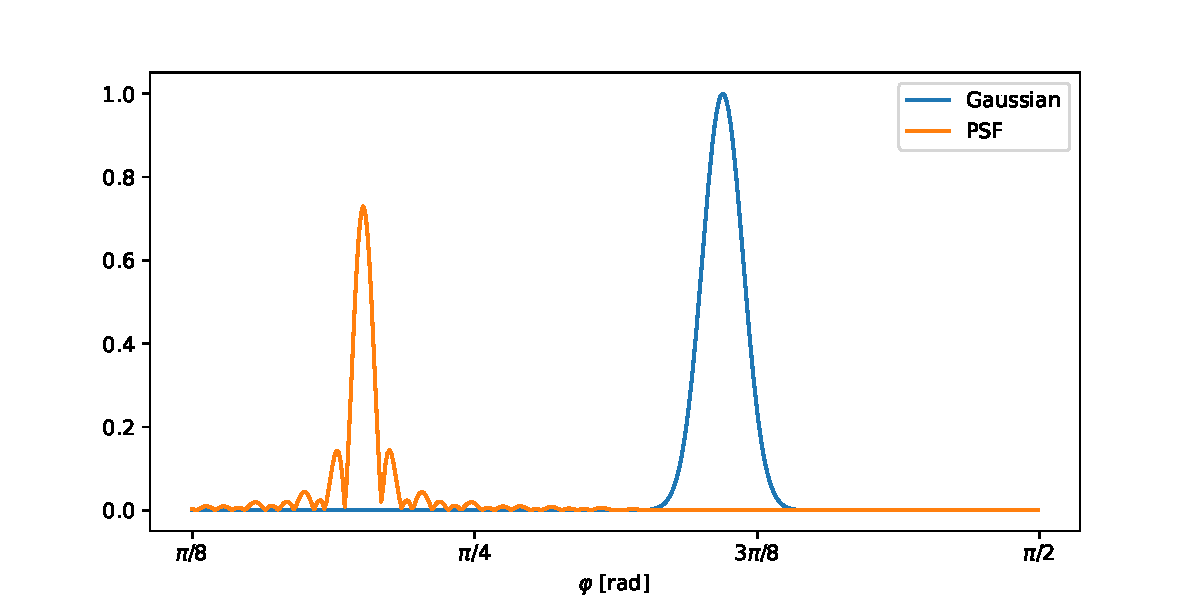
\includegraphics[width=1.0\textwidth]{pics/PSF_cut_image.pdf}
		\caption{A cut through a Gaussian profile and a PSF along the angular direction. Both profiles are rotationally symmetric.}
		\label{fig:PSF_cut_image}
\end{figure}
\begin{figure}[H]
	\centering
		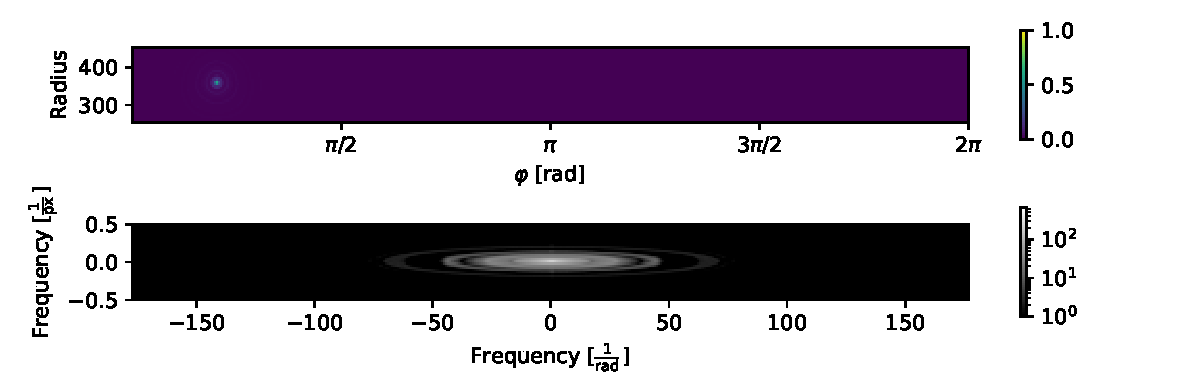
\includegraphics[width=1.0\textwidth]{pics/PSF_fourier.pdf}
		\caption{An image with a PSF (top) is transformed into the frequency space (bottom).}
		\label{fig:PSF_fourier}
\end{figure}
\begin{figure}[H]
	\centering
		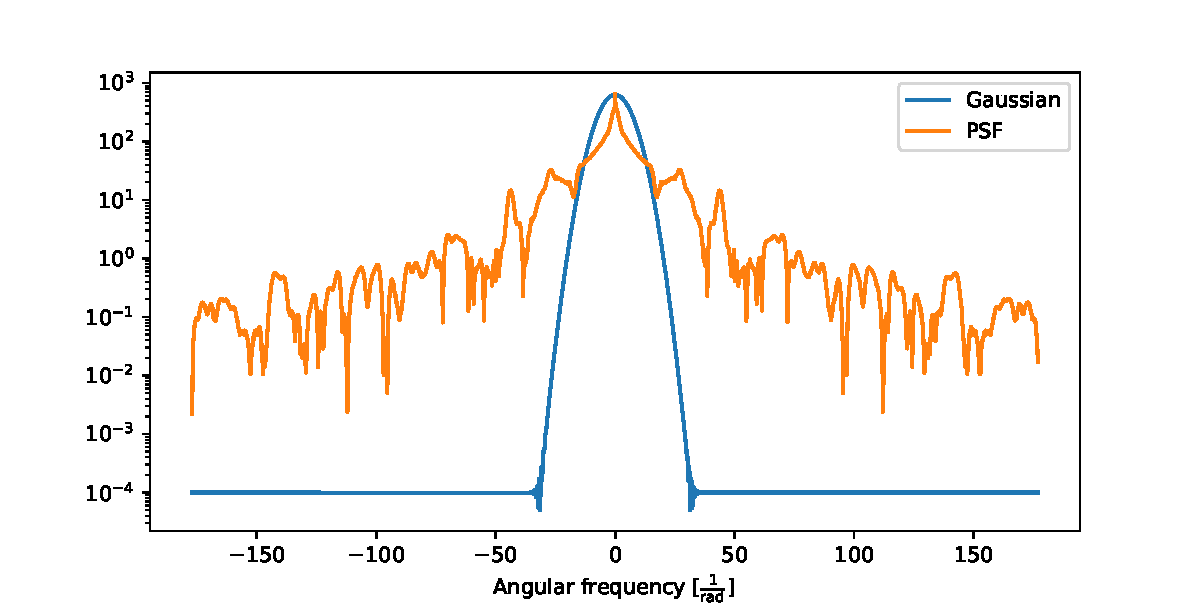
\includegraphics[width=1.0\textwidth]{pics/PSF_cut_fourier.pdf}
		\caption{The Fourier transform of a Gaussian profile and a PSF at radial frequency zero. }
		\label{fig:PSF_cut_fourier}
\end{figure}
